\documentclass[11pt]{article}
\usepackage[letterpaper,margin=0.92in]{geometry}
\usepackage[T1]{fontenc}\usepackage{lmodern,amsmath,amssymb,amsthm,booktabs,array,tabularx,longtable,enumitem,microtype,fancyhdr,tikz}
\usetikzlibrary{arrows.meta,positioning}
\usepackage[hidelinks]{hyperref}
\setlength{\parindent}{0pt}\setlength{\parskip}{5pt}\setlist{nosep}
\newtheorem{theorem}{Theorem}[section]\newtheorem{proposition}[theorem]{Proposition}\newtheorem{lemma}[theorem]{Lemma}\newtheorem{corollary}[theorem]{Corollary}
\theoremstyle{definition}\newtheorem{definition}[theorem]{Definition}\newtheorem{example}[theorem]{Example}\newtheorem{conjecture}[theorem]{Conjecture}
\newcommand{\Q}{\mathbb Q}\newcommand{\N}{\mathbb N}\newcommand{\R}{\mathbb R}\newcommand{\E}{\mathbb E}\newcommand{\Prb}{\mathbb P}\newcommand{\Dep}{\operatorname{Dep}}\newcommand{\Ind}{\operatorname{Ind}}\newcommand{\Vfy}{\operatorname{Verify}}\newcommand{\supp}{\operatorname{supp}}\newcommand{\Fix}{\operatorname{Fix}}\newcommand{\eps}{\varepsilon}
\pagestyle{fancy}\fancyhf{}\fancyhead[L]{\small Search Dynamics to SICs}\fancyhead[R]{\small\partlabel}\fancyfoot[C]{\thepage}\setlength{\headheight}{14pt}
\newcommand{\status}[1]{\textbf{Status.} #1}
\newcommand{\partlabel}{Part I / Atlas repeat audit}
\title{From Search Dynamics to Semi-Ideal Computers\\[5pt]\large Part I: Theorem Mazes, Certified Settlement, and Feedback Control\\\normalsize Corrected research edition v0.5 / Atlas repeat audit}
\author{Brian Tenneson, original research and research direction\\Picard (AI-assisted mathematical revision)}
\date{26 November 2026 (Atlas repeat audit)}
\begin{document}\maketitle
\begin{abstract}
Automated theorem proving is modeled as navigation through an implicit, verifier-backed directed graph. This corrected edition distinguishes native proof cost, route cost, and the total effort of discovering a route; separates object-level proof/refutation from metalogical dependence/independence; and supplies sufficient conditions for safe compression, completeness, and stochastic discovery control. A cumulative verified ledger induces a semi-ideal computer (SIC) without necessarily determining the operational dynamics. Bellman values induce expected Abel translation on preterminal trajectories, but properness is essential: a zero-cost loop can satisfy Bellman equations without discovering anything. We develop explicit finite-state hypotheses, counterexamples, certificate contracts, and an experimental design that preserves the original negative results. The historical measurements are reproduced as reported, not independently replicated. No universal acceleration, universal decision procedure, or unrestricted self-certification is asserted.
\end{abstract}
\textbf{Edition note.} This is a substantive reconstruction of the supplied 48-page v0.4a PDF, not a line-by-line typesetting of unavailable original source. It retains its mathematical program, historical numerical tables, conjectural themes and negative controls, while reorganizing the arguments and adding proofs and counterexamples. The original is an archival predecessor, not the authority for the corrected definitions. The companion Part II uses only the explicitly stated results and hypotheses of this edition. No operational software upgrade is implied.
\clearpage\tableofcontents\clearpage
\section{The program: reduce the maze before learning to navigate it}
The underlying idea of the August 14, 2026 manuscript, audited September 29, is that the main obstacle to mathematical discovery is often not the shortest-path computation on an explicit graph but the generation of that graph. A short formal problem may induce an enormous, even infinite, collection of legal states. The task is to expose as little of this collection as possible while preserving the verifier's authority. The original hierarchy remains useful as a research judgment, not a theorem of efficiency.
\begin{center}
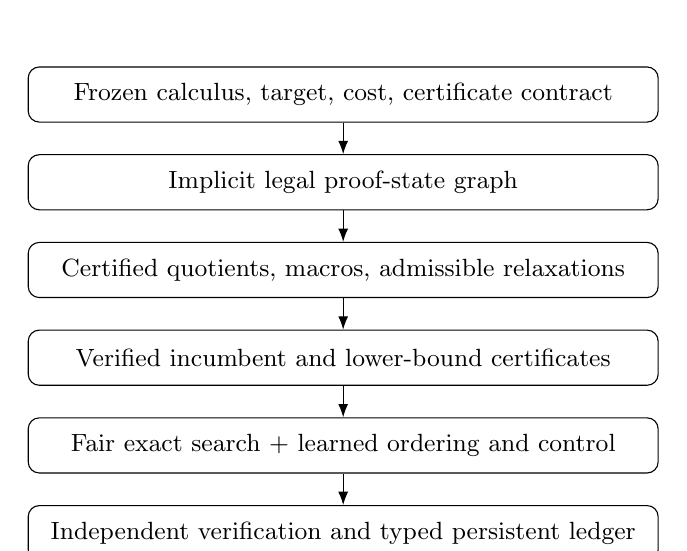
\begin{tikzpicture}[node distance=4mm, every node/.style={font=\small}, b/.style={draw,rounded corners,minimum width=8cm,minimum height=7mm,align=center},>=Latex]
\node[b](a){Frozen calculus, target, cost, certificate contract};
\node[b,below=of a](b){Implicit legal proof-state graph};
\node[b,below=of b](c){Certified quotients, macros, admissible relaxations};
\node[b,below=of c](d){Verified incumbent and lower-bound certificates};
\node[b,below=of d](e){Fair exact search + learned ordering and control};
\node[b,below=of e](f){Independent verification and typed persistent ledger};
\foreach \x/\y in {a/b,b/c,c/d,d/e,e/f}{\draw[->] (\x)--(\y);}
\end{tikzpicture}
\end{center}
Priorities: first exploit exact equivalences and partial-order reductions; then admissible abstractions, branch-and-bound and Horizon certificates; then verified compilation and reusable landmarks; use min-plus algebra as the common cost language; finally test learned ordering, Hilbert locality, portfolio scheduling, and dynamical representations. A reduction that costs more than it saves is not an acceleration. A heuristic that discards an unexamined branch is not a certified reduction.
\section{Theorem mazes and the three costs}
Fix a calculus $F$, hypotheses $\Gamma$, target $\varphi$, and a declared certificate checker. The complete operational state may contain pending subgoals and contexts, variable assignments, available formulas, resource counters, and any information that changes future legal moves. In forward search a state $p$ can be the set of already available formulas when that set suffices for legality. A $k$-premise rule deriving $\beta$ from premises in $p$ becomes one edge $p\to p\cup\{\beta\}$. Individual formulas alone require a hypergraph or equivalent incidence representation. Backward search needs the full residual goal state. The target is a verifier-accepted certificate, not just a plausible formula.
\begin{definition}[Weighted maze]
$G=(V,E,s,Z,w)$ is a directed multigraph with entrance $s$, verified exits $Z$, and exact rational nonnegative edge costs $w:E\to\Q_{\ge0}$. A legal finite walk $P$ has cost $w(P)=\sum_{e\in P}w(e)$. Define $d(v,Z)=\inf_{P:v\leadsto Z}w(P)$, with $\inf\varnothing=\infty$. Zero-length walks are permitted at exits. In a finite graph, every finite distance is attained by a simple path (delete nonnegative cycles).
\end{definition}
\textbf{Three distinct currencies.} Native proof cost counts the transparent primitive derivation. Route cost counts declared operations along a successful trajectory. Discovery effort includes failed branches, candidate generation, verification, bookkeeping, and scheduling. A macro may reduce route cost while leaving native proof cost unchanged. An algorithm can return an optimal route after exponential discovery effort. Exact rational arithmetic prevents rounding mistakes, not state explosion. A natural-number naming scheme for rational weights is an optional encoding, not a fractional logical inference; the latter would require an independent semigroup law $\Phi_{s+t}=\Phi_s\circ\Phi_t$.
\begin{center}\small
\begin{tabularx}{\linewidth}{l l X}\toprule
Algorithm & Explicit graph operations & Guarantee / restriction\\\midrule
BFS & $O(n+m)$ & Minimum unit edge count; finite/exhaustible layers\\
DFS & $O(n+m)$ & Reachability on finite graphs, not optimal cost\\
Dijkstra & $O((n+m)\log n)$ & Nonnegative weights with indexed binary heap; array $O(n^2+m)$\\
DAG shortest path & $O(n+m)$ & Known topological order, finite graph\\
Floyd--Warshall & $O(n^3)$ & All pairs, explicit finite graph\\
A* & instance dependent & Admissible bounds, correct reopening/dominance and stopping\\\bottomrule
\end{tabularx}\end{center}
These are graph operation bounds, not exact bit complexity or wall-clock guarantees. In an implicit tree with branching factor $b>1$ and solution depth $d$, exhaustive breadth-first generation may cost $O(b^d)$ nodes; depth-first generation to depth $\ell$ may cost $O(b^\ell)$ time. If there are infinitely many zero-cost states, uniform-cost search can starve a positive-cost solution. Example: $s\to z$ costs 1, while $s\to x_1\to x_2\to\cdots$ costs zero. Every finite zero-cost expansion precedes $z$. Even positive rational edges can accumulate below 1 (use $2^{-j-1}$). A useful sufficient condition is effective finite branching and a uniform positive lower bound on edge costs, which makes bounded-cost tree layers finite. For reachability alone use fair enumeration regardless of cost. Hilbert-style ordering may rank states but neither creates a legal edge nor provides a lower bound.
\section{Transfer and certificate soundness}
\begin{theorem}[Cost-preserving maze transfer]
Suppose a search problem and a maze admit effective decoding of each reachable graph walk into a legal transaction sequence of exactly the same declared route cost, and every admissible transaction sequence has a graph representation with that same cost. Exits decode to independently accepted certificates of the requested type, and every such reachable terminal transaction has an exit representation. Then any returned graph exit decodes to a sound settlement relative to the checker. If the graph algorithm is correct for the represented graph and finds a minimum-cost exit walk, the decoded route has minimum declared route cost.
\end{theorem}
\begin{proof} Soundness is the decoding and checker hypothesis. If a cheaper admissible route existed, its graph representation would be a cheaper exit walk, contradicting optimality. Cost preservation in both directions is essential. Decoding alone only proves optimality among represented routes, and a decoder that changes cost need not even preserve the ordering of represented routes. No statement about total search work follows.\end{proof}
For example, consider two graph exit routes of costs 1 and 2 and legal transaction routes of costs 1 and 2. Even if every transaction route has a cost-matching encoding, a decoder that swaps the two routes returns cost 2 from the graph optimum of cost 1. This is excluded by the repaired hypothesis. A pruned or bounded maze must state whether its optimum is relative to its scope or global in the original calculus. The latter requires a preservation proof. A sound certificate checker can be incomplete for a chosen target class; no failed search may be converted into a negative theorem by changing the label on a timeout.
\section{Exact reductions before learning}
\subsection{Novelty and the operational quotient}
Let $B(x)$ be the verified bank projection. Strictly increasing transitions $B\subsetneq B'$ define an acyclic graph of novelty. But a complete state can revisit a queue, discard a proposal, or restart without changing $B$. A novelty DAG is not automatically the entire search space. If two states have the same bank but only one has retained a promising queued inference, merging them can lose a reachable exit under a constrained controller.
\begin{theorem}[A sufficient exact quotient contract]
Let $\sim$ be an effectively decidable equivalence on reachable complete states. Require exit status to be class-invariant. For each $x\sim y$ and each edge $x\to x'$ of cost $c$, require an effectively selectable edge $y\to y'$ of cost $c$ with $x'\sim y'$, and conversely. Require an exit witness to be recoverable from each reached exit representative. Then quotient walks from $[s]$ lift to walks from $s$ of the same cost, and concrete walks project at the same cost. Distances to exits are equal, including $\infty$. This is a structural guarantee; using a particular graph algorithm on an implicit quotient also requires its effective successor-generation and termination hypotheses.
\end{theorem}
\begin{proof} Construct the quotient with edges labeled by class pair and cost. Project each concrete edge. To lift a quotient walk inductively, match a representative witnessing the next quotient edge to the current concrete state via the stipulated condition. Exit invariance and witness recovery finish the lifting. Taking infima both ways proves equality.\end{proof}
This sufficient contract can be stronger than necessary. Partial-order reductions need their own commutation and dependency proofs; stochastic controllers additionally need compatible transition distributions and costs if expected values are to be preserved. Ledger equality alone meets none of these requirements automatically.
\subsection{Conservative macros and reuse}
A certified macro edge is a finite sequence of native legal steps with an explicit expansion that passes the original checker. Adding such edges preserves theoremhood, provided the hypotheses and contexts are retained. With macro cost equal to native expansion cost, it also preserves optimal native route cost by expansion in both directions. With smaller declared transaction cost, optimal transaction cost can decrease but cannot be compared as native proof cost. A useful accounting criterion for repeated use is $k(a-b)>C$, where $a$ is cost of recomputation, $b$ includes retrieval and checking, $C$ is the one-time certified compilation cost, and $k$ is the number of uses. This elementary inequality is a model of when reuse pays; actual costs may vary with context.
\subsection{Admissible relaxation and label pruning}
\begin{proposition}[Lower bound and incumbent]
If every concrete exit walk from $v$ projects to an abstract exit walk from $\pi(v)$ of no greater cost, the abstract distance $h(v)$ is a lower bound on $d(v,Z)$. If a verified incumbent costs $B$, a reached path-label $(v,g)$ cannot improve it whenever $g+h(v)\ge B$.
\end{proposition}
\begin{proof} Infimize the path-relaxation inequality over concrete walks. Every extension of the represented label costs at least $g+h(v)$.\end{proof}
Global vertex deletion additionally needs a valid cost-to-come dominance rule. For example an expensive arrival with $g=9$ and $h(v)=2$ cannot improve $B=10$, but a later arrival with $g=1$ may. Prune labels, not all future visits, unless the relevant state is complete and dominance is established. When enumerating all optimal proofs rather than only strictly improving a known incumbent, equality cannot be pruned indiscriminately. A learned estimate is not admissible merely because its test error is small.
\section{Min-plus algebra and safe navigation}
On finite graphs the semiring $(\Q_{\ge0}\cup\{\infty\},\min,+)$ describes alternative and sequential route costs. On infinite graphs an infimum of rational path costs can be irrational; use $[0,\infty]$ for arbitrary infima or impose an attainment hypothesis. A concrete path is an upper-bound witness; an admissible relaxation is a lower-bound witness. Neither is the other. Learned scores may rank a frontier, select a portfolio, or estimate probability of settlement by budget, but may not veto a legal branch without a certificate of irrelevance.
\begin{proposition}[Fair background completeness]
Suppose there is an effective enumeration of all finite candidate certificates, a verifier halts on each candidate, and each completed enumeration-and-check step advances the enumeration and deposits any accepted target certificate. Assume the run may halt only after the declared target is accepted, or continues indefinitely; on every infinite run the background enumerator receives infinitely many completed steps. If an accepted target certificate occurs in the enumeration, the run eventually accepts a target certificate. If the run instead continues forever and retains every accepted certificate, every enumerated accepted certificate is eventually deposited.
\end{proposition}
\begin{proof} If a run has not already accepted a target and halted, it cannot halt prematurely by hypothesis. An infinite run tests every finite-index candidate, so in particular it tests the promised accepted target. This contradicts an infinite run that never accepts a target. In the continuing variant, the same finite-index argument applies to each accepted certificate. A finite-budget stop with status $U$ is not covered by the eventual-success guarantee.\end{proof}
This is a semidecision guarantee on a declared enumerable certificate language, not completeness for arbitrary semantic truths or independence. For example, a fixed positive share of verifier calls works only if candidate production itself is fair and no individual call blocks permanently. Timeouts must dovetail longer attempts if the checker is not total. The Part II design exploits this division of labor.
\section{The theoremhood quotient and Proof Horizon}
For a fixed $F,\Gamma,\varphi$, let $\mathcal P_\varphi$ be the set of verifier-accepted proof tours. On this set define $P\sim_\varphi Q$ for every pair. If nonempty, the quotient $\mathcal P_\varphi/\sim_\varphi$ contains exactly one element, the equivalence class $[P]=\mathcal P_\varphi$. The class, not the quotient-of-classes, contains the concrete paths. The original Corollary 6.3 used $P\in C_\varphi$ after defining $C_\varphi$ as the quotient; the corrected Horizon is
\[H_w(\Gamma,\varphi)=\inf_{P\in\mathcal P_\varphi}w(P),\quad H_w=\infty\text{ if }\mathcal P_\varphi=\varnothing.\]
For unit native costs, the infimum over a nonempty set is a minimum by well-ordering. A finite graph also attains its optimum. Infimum attainment is not automatic for rational weights on infinite graphs. The theoremhood quotient is a semantic endpoint; recognizing an unexplored path as a proof requires verifying it. It is not itself a search reduction.
\section{Verified transition systems and SICs}
A controlled operational machine consists of complete states $X$, legal transformations or transition kernels, a scheduler, an independent verifier, and a universe $\mathcal R$ of typed records. The complete state $X_t$ may be nonmonotone. Let $\iota$ inject admitted inputs into a disjoint typed record space. For stages numbered from 1 let $V_1=\varnothing$ and let $V_n$ be the newly accepted records on entering stage $n$. Define
\[ C(\Gamma,n)=\iota(\Gamma)\cup\bigcup_{j=1}^n V_j.\]
Given a declared target predicate on records, $Z_{\mathcal R}$, define $H(\Gamma,n)=1$ iff $C(\Gamma,n)\cap Z_{\mathcal R}\ne\varnothing$. Freeze the target-specific computation and extend it constantly after the first hit. The initial inputs must be checked or explicitly designated assumptions, never confused with derived theorems. If an input already carries the target certificate, immediate halt is permitted unless the SIC variant explicitly excludes it.
\begin{theorem}[Cumulative-history SIC lift]
Under persistent typed records and the constant extension convention, the pair $(C,H)$ has the stated SIC properties: initial input, increasing verified history, persistent halting and post-halting freezing.
\end{theorem}
\begin{proof} $C(\Gamma,1)=\iota(\Gamma)$ and $C(\Gamma,n+1)=C(\Gamma,n)\cup V_{n+1}$. Membership of an accepted terminal record persists by inclusion. The stopped extension is constant by definition.\end{proof}
This is a runwise construction. A stochastic or nondeterministic system gives a family of SIC traces indexed by randomness or scheduling; a deterministic stage map needs those inputs fixed. An effective ATP additionally requires effective generation, verification, soundness and eventual success on the promised derivable target class. Monotonicity alone does not imply those conditions. Persistent verified records can include proof objects and provenance, not merely formulas. Corrections to a faulty checker version require a new versioned contract and explicit invalidation/rechecking, not silent deletion.
\section{ATP, ALD and AMLD: the corrected logical typing}\label{sec:types}
This section is an explicit correction to the inconsistent use of the AMLD name in the original control sections. We use the nested metalogical convention: an ATP searches a derivation; an ALD settles an object-level question with appropriate certificates; an AMLD settles the metaproposition of dependence versus independence. An implementation may contain many agents, but their names are not its mathematical output alphabet. No new sovereignty or game layer is needed.

Fix a recursively enumerable, classical object theory $G$ and sentence $\varphi$, and declare a metatheory $M$ that can express the relevant proof predicates. Assume the designated proof checker and translations are sound relative to their stated semantics. Actual truth of a certified metaproposition requires the relevant soundness of $M$; mere derivability in $M$ is the syntactic output contract, not an unconditional truth guarantee. The following predicates are typed:
\[ P_G(\varphi):=\exists p\,\operatorname{Prf}_G(p,\varphi),\quad R_G(\varphi):=\exists p\,\operatorname{Prf}_G(p,\neg\varphi),\]
\[ \Dep_G(\varphi):=P_G(\varphi)\lor R_G(\varphi),\qquad \Ind_G(\varphi):=\neg\Dep_G(\varphi).\]
The proof predicate is an explicitly declared effective syntax or certificate relation; where axiom membership is only enumerable, witnesses of axiom enumeration are included. An accepted object proof can supply a dependence certificate via a verified metalevel translation. An independence certificate is a metatheoretic proof of $\Ind_G(\varphi)$ under the declared interpretation, or a certified semantic construction with a proved bridge to nonderivability. A model of $G+\neg\varphi$ alone establishes at most nonderivability of $\varphi$ assuming the appropriate soundness bridge; it does not also establish nonderivability of $\neg\varphi$.
\begin{center}\small
\begin{tabularx}{\linewidth}{l l X}\toprule
Interface & Result & Accepted meaning\\\midrule
ATP & proof & $G\vdash\varphi$, checked derivation\\
ALD & $P,R$ & $G\vdash\varphi$ or $G\vdash\neg\varphi$\\
ALD (extended) & $I$ & Relays accepted metalogical independence evidence\\
AMLD & $D,I$ & $M\vdash\Dep_G(\varphi)$ or $M\vdash\Ind_G(\varphi)$\\
Diagnostic channel & $C$ & Checked inconsistency/conflict, identifying theory and evidence\\
All interfaces & $U$ & No accepted settlement at declared stopping budget\\\bottomrule
\end{tabularx}\end{center}
$C$ and $U$ are explicitly typed diagnostic/nonsettlement statuses, not extra alternatives to a well-formed dependence-versus-independence query. The internal search may have P, R, D, I and C workers; the AMLD's mathematical question remains $D$ versus $I$. The outer ALD can display an $I$ obtained from the nested AMLD. If $M$ certifies dependence nonconstructively without an object proof witness, the outer ALD must not infer a particular $P$ or $R$ from that fact alone. Under a consistent classical $G$, object-level $P$ and $R$ cannot both occur. In an inconsistent $G$ both may occur, and dependence may be true; $C$ is not a synonym for independence. If the metatheory certifies both $D$ and $I$, the records signal metatheoretic inconsistency or a verification/translation failure, rather than permission to select either as trustworthy.
\begin{theorem}[No settlement from silence]
Under the certificate interface alone, a finite failed proof/refutation search is not a general certificate of independence. A finite failed metatheoretic search, without additional information about the search scope or a certified decision procedure, is not a general certificate of either dependence or independence.
\end{theorem}
\begin{proof} The interface permits bounded runs that spend their entire budget on unsuccessful candidates or other legal search work. Take a classical first-order language with a unary predicate $P$ and constant $c$. For the empty nonlogical theory, the sentence $P(c)$ is independent: singleton structures interpreting $P$ as respectively full and empty establish both nonderivability statements by soundness. For the theory with axiom $P(c)$ the same sentence is derivable. A bounded run permitted to defer the relevant certificate can return $U$ in either case. In a metatheory able to formalize these finite model arguments and the elementary proof, dependence and independence have respective certificates on the two instances, yet the interface allows both searches to stop before accepting them. Thus $U$ alone does not imply either mathematical status across the permitted runs and theories. This is not a claim that every fixed scheduler can delay every certificate, nor that the complete input and trace of a particular run cannot yield more information.\end{proof}
The result is an observation about the interface, not an impossibility of bounded exact decision on suitably decidable classes. A finite exhaustive search can certify absence within its scope; a theorem extending that absence to all proofs is a separate obligation.
\section{Halting, fixed points and reflection}
Let $T:X\to X$ be a deterministic complete-state update, $S$ the set of certified terminal states. If $T(x)=x$ for $x\in S$ and $T(x)\ne x$ for $x\notin S$, then $\Fix(T)=S$ by the two inclusions. A nonterminal counter increment can enforce the latter assumption, but it must be frozen on halting; a ledger projection can be fixed while the full machine continues. A stochastic absorbing set need not consist of pointwise fixed states unless each terminal transition is the corresponding point mass. Existence of a fixed point says nothing about reachability from a particular entrance or expected time.

Reflection: if a frozen machine code $\langle M_0\rangle$ and its predicates are expressible in a background theory $M$, an effective prover complete for derivable targets in that theory can enumerate proofs of expressible derivable properties of the code. Examples are finite scheduler fairness, checker invariants, or bounded Horizon statements. This follows directly from the declared completeness assumption, not a new general self-certification theorem. Such a proof is relative to $M$. G\"odel, Church and Tarski limits still apply; no proof of unrestricted semantic truth, global self-soundness, or general decidability follows. The set generated by finite nonempty compositions of a nonempty family of endomorphisms is a semigroup (adjoin the identity if a monoid is wanted); an iterated function system with contraction or a continuous/fractional flow requires its own conditions.
\section{Feedback control with a genuine settlement objective}
Let $X_t$ be complete operational states, $S$ a prospectively observable absorbing set, $a_t$ an action chosen using the available history, and $K(\cdot\mid x,a)$ a declared transition kernel. Use a pre-transition filtration $\mathcal F_t$ including the current state and chosen action (and any randomization used to select it), with $X_{t+1}$ conditionally distributed according to $K(\cdot\mid X_t,a_t)$. Let $\tau=\inf\{t:X_t\in S\}$. A finite-horizon objective is $\Prb_x^\pi(\tau\le B)$ for a step budget. Cost budgets are separate. For total nonnegative cost, either restrict to proper policies that reach $S$ almost surely with finite expected cost, prove that the minimizing policy is proper, or declare a failure convention that excludes nontermination from successful settlement. A finite failure penalty by itself need not force termination. Without a properness or successful-hit contract, $\E\sum_{t<\tau}c(X_t,a_t)$ can be small precisely because a machine does nothing forever.
\begin{theorem}[Additive drift with explicit stopping]\label{thm:drift}
Assume $D\ge0$, $D=0$ on $S$, $\E D(X_0)<\infty$, and $D(X_{t\wedge\tau})$ is integrable at every finite time. If $\E[D(X_{t+1})-D(X_t)\mid\mathcal F_t]\le-\mu$ on $t<\tau$, with $\mu>0$, then $\E\tau\le\E D(X_0)/\mu$, hence $\tau<\infty$ almost surely.
\end{theorem}
\begin{proof} Apply conditional expectation to the stopped process. On $t\ge\tau$ its change is zero. Telescoping gives $0\le \E D(X_{n\wedge\tau})\le\E D(X_0)-\mu\E(n\wedge\tau)$. Monotone convergence gives the result; no unproved infinite-time optional stopping identity is needed.\end{proof}
If an ideal action decreases $D$ in expectation by at least $\alpha$, and a learned action loses at most $\eps<\alpha$ at every nonterminal reachable state, apply Theorem~\ref{thm:drift} with $\mu=\alpha-\eps$. A positive aggregate drift across a dataset is not a substitute for this conditional guarantee. If $X_0$ is random, the right side is its expected initial potential (the old text used $D(X_0)$ without specifying a fixed start).
\begin{proposition}[Finite-horizon progress tail]
For deterministic $B\in\N$ let $Y_t$ be integrable square-integrable progress increments with $\E Y_t=\mu$ and $\operatorname{Var}(\sum_{t=1}^B Y_t)\le B\sigma^2$. If $B\mu>D_0$, then
\[\Prb\left(\sum_{t=1}^B Y_t<D_0\right)\le\frac{B\sigma^2}{B\sigma^2+(B\mu-D_0)^2}.\]
\end{proposition}
\begin{proof} Cantelli's inequality for the centered sum, whose variance is bounded as stated, gives the claim. Independent increments with common variance suffice; a martingale-difference decomposition suffices if the conditional drift is constant and the innovations have total second moment at most $B\sigma^2$.\end{proof}
The threshold must be linked to actual settlement to bound failure probability. In an absorbing experiment, increments after the stop are usually zero, so common unconditional means through $B$ are not automatic. A separate direct bound from Theorem~\ref{thm:drift} is $\Prb(\tau>B)\le\E D(X_0)/(\mu B)$ for $B>0$.
\subsection{Allocating resources to typed searches}
Use object-level proof/refutation and metalogical dependence/independence frontiers with typed consistency monitoring. An equal resource floor is not the same as fairness over individual candidates. Let $r_i\ge0$, $\sum_i r_i=R>0$. Suppose the objective is an additive differentiable concave response $H(r)=\sum_i h_i(r_i)$, with finite right derivatives at zero. Then a maximizer exists on the compact simplex when the responses are continuous, and its KKT conditions are $h_i'(r_i)=\lambda$ on active agents, $h_i'(0)\le\lambda$ otherwise. These conditions are also sufficient by the concavity supporting-line inequality. This is a model of resource allocation, not a theorem that actual probabilities add. For independent success events with probabilities $p_i$, the probability of any success is $1-\prod_i(1-p_i)$, and dependent events require joint information. Additive hazards can be a separate model with explicit assumptions. Any completeness-critical floor must be imposed before optimizing remaining resources.
\section{Discovery as a verifier-backed event}
A new verified record $q$ is weakly novel at time $t$ if $\Vfy(q)=1$ and its equivalence class is absent from the \emph{pre-deposit} ledger $B_t$. The novelty relation must preserve the intended record semantics. Define an online discovery event by a frozen observable criterion. An operationally useful discovery requires additional evaluation: given workload distribution $\nu$, policy $\pi$, budget $R$ and penalty $\kappa>0$, let $J_R(C,x)$ equal measured cost to successful settlement if it occurs within $R$, and $R+\kappa$ otherwise (including nontermination). Define
\[U_R(q\mid x)=\E_{C\sim\nu,\,\pi}[J_R(C,x)-J_R(C,x\oplus q)].\]
Here the expectation includes controller randomness, and $x\oplus q$ uses the verified interface with retrieval/checking overhead charged. Weak novelty plus $U_R>0$ is one prospective definition of operational usefulness, but its label may only be known retrospectively. An estimated positive sample mean is not a proof of positive population effect. Online stopping must use immediately observable acceptance or a separately modeled delayed evaluation state.

The source's finite-horizon ``hazard'' is more precisely a cumulative hitting probability. Conditional on the current history and survival, use $h^\pi(x;R)=\Prb^\pi_x(\tau<\infty,\tau\le R)$ for steps, and $\Prb^\pi_x(\tau<\infty,\sum_{t<\tau}c_t\le R)$ for cost. Explicit $\tau<\infty$ prevents zero-cost nontermination from counting as discovery. A discrete hazard at time $j$ is instead $\Prb(\tau=j\mid\tau\ge j)$ when the conditioning event has positive probability. Policy-relative discovery depth is the infimum of declared costs of admissible finite successful trajectories; in finite/discrete stochastic models one may require positive trajectory probability. For continuous state spaces, individual paths can have probability zero; specify a support-based reachability notion before using this definition. A low best-case depth need not imply a low expected discovery cost.

Readiness features may include novelty of proposals, residual-goal changes, representation shifts, lemma transfer, compression, and cross-approach reuse. Online features must be available before the decision: later usefulness and later successful transfer are labels, not current predictors. Mechanism labels such as quotient, duality, decomposition, generalization, composition and representation change are descriptive unless a causal comparison supports their use. Motifs and semigroup compositions produce candidate transformations; no analogy to musical transposition establishes logical legality. Every candidate must cross the original verifier boundary.
\section{The Bellman--Abel repair}\label{sec:abel}
The source's Proposition 22.1 is algebraically correct conditional on its Bellman equation. The gap is in using an undiscounted nonnegative accumulated cost as a discovery objective without a properness contract. In a state $x$, let an action stay at $x$ forever for cost zero and another move to a terminal $z$ for cost 1. The unrestricted accumulated cost infimum is 0; the value among terminating policies is 1. Moreover the Bellman equation $v(x)=\min\{v(x),1\}$ has every nonnegative solution $v(x)\in[0,1]$ (with $v(z)=0$), so it is not uniquely characterized by the equation. Even the proper-policy value permits the improper loop as a minimizing action. A separate progress condition is indispensable. We retain zero costs for graph analysis but use the following sufficient contract for stochastic control.
\begin{theorem}[Finite positive-cost discovery]\label{thm:ssp}
Let $X$ be finite with nonempty finite action sets at every nonterminal state, a fixed Markov kernel, and all history-dependent randomized policies admissible. Let terminal states be absorbing, with cost zero at terminals, and $0<c_0\le c(x,a)\le c_1<\infty$ elsewhere. Assume there exists a policy of finite expected total cost from every state. For $V^*(x)$ the infimum of expected accumulated preterminal cost over all admissible policies, $V^*$ is finite, nonnegative and satisfies
\[V^*(x)=\min_a\{c(x,a)+\E[V^*(X')\mid x,a]\},\qquad V^*|_S=0.\]
Every stationary minimizing selector reaches $S$ almost surely, with expected hitting time at most $V^*(x)/c_0$, and attains $V^*(x)$.
\end{theorem}
\begin{proof}
Finiteness follows from the assumed policies. One-step conditioning on the chosen action shows that every continuation costs at least the statewise infimum, proving the lower inequality. For each successor select a policy within $\eps$ of the infimum, concatenate after a minimizing first action, and let $\eps\downarrow0$ for the reverse inequality. Finite action sets ensure attainment of the minimum. Under a minimizing selector, conditional expected decrease of $V^*$ equals $c(x,a)\ge c_0$ before termination. Theorem~\ref{thm:drift} gives the hitting-time bound. Telescope the Bellman equality up to $n\wedge\tau$; boundedness of $V^*$ on finite $X$ and almost-sure termination imply $\E V^*(X_{n\wedge\tau})\to0$. Nonnegative costs and monotone convergence yield equality of actual expected cost and $V^*(x)$.
\end{proof}
If zero-cost transitions are essential, use a properness proof for the selected policy, a separately certified decreasing rank or a lexicographic time penalty, rather than importing this theorem unchanged. The theorem is a finite stochastic shortest-path specialization, consistent with established theory \cite{ssp}. It is not claimed as a new general result in dynamic programming.
\begin{corollary}[Expected Abel translation]
Under Theorem~\ref{thm:ssp}, put $A^*=-V^*$. Before discovery,
\[\max_a\{\E[A^*(X')-A^*(x)\mid x,a]-c(x,a)\}=0.\]
Every minimizing selector attains equality. For unit costs the expected increment is one. For a deterministic transition the equality is pathwise along the selected preterminal edge.
\end{corollary}
\begin{proof} Negate the Bellman equality and subtract $A^*(x)$.\end{proof}
The terminal stopping rule is essential. No nonzero Abel translation can hold at an absorbing fixed point or around a deterministic directed cycle of positive total cost. Also a functional equation $A(Tx)=A(x)+1$ is a semiconjugacy on its domain, not necessarily a conjugacy unless $A$ is injective with an appropriate inverse. Stochastic conditional translation is not a sample-by-sample constraint.
\subsection{Residuals, action gaps and approximate control}
For a frozen candidate $\widehat A$, define $s_a(x)=\E[\widehat A(X')-\widehat A(x)\mid x,a]-c(x,a)$ and the statewise residual $\rho(x)=-\max_a s_a(x)$. The realized residual $\widehat A(X_{t+1})-\widehat A(X_t)-c_t$ decomposes into $s_{a_t}(X_t)$ plus innovation $\eta_{t+1}=\widehat A(X_{t+1})-\E[\widehat A(X_{t+1})\mid\mathcal F_t,a_t]$. The latter has conditional mean zero under the declared kernel; innovation variance is distinct from coordinate error.
\begin{proposition}[Action-gap and regret bounds]
If each estimated action score differs from its exact score by at most $\eps$, a greedy estimated action loses at most $2\eps$ in true score. If the true best action is unique and separated by a gap strictly larger than $2\eps$, it is selected.
\end{proposition}
\begin{proof} Compare the two maximizing inequalities: the true best score is at most its estimate plus $\eps$, at most the greedy estimate plus $\eps$, at most the greedy true score plus $2\eps$.\end{proof}
A uniform value error $\|\widehat A-A^*\|_\infty\le\delta$ implies score error at most $2\delta$ for an exact kernel. Because the current-state term is common to all actions, greedy action regret can in fact be bounded by $2\delta$ by comparing only successor expectations minus cost. In Theorem~\ref{thm:ssp}, if this regret is below $c_0$, exact-value expected decrease remains positive under the learned policy and Theorem~\ref{thm:drift} applies. If transition expectations are themselves estimated, their errors must be included. Held-out average errors are not uniform certificates.

A local Abel score improvement over baseline is a graded proxy, not a finite-budget causal gain. A deterministic path loss should only impose translation on transitions known to be optimal (or explicitly chosen and separately justified as productive for that coordinate). On stochastic samples, fit conditional means or Bellman residuals rather than demanding a unit increment on every transition. A fixed policy can have its own value coordinate; a single scalar does not automatically generalize across calculi or controllers. Section~\ref{sec:protocol} retains prospective testing.
\section{Preserved evidence: settlement-compass experiments}
\status{Historical report from v0.4a, not newly replicated or independently validated.} Experiments 001--003 were exploratory diagnostics. Experiment 004 froze one eligible universe, a sealed 20-target test set and a nested training ordering. Training from scratch used the same features, negatives, test pools, seeds and model class. The MAX condition used 3,612 roots. Table~\ref{tab:shells} reproduces the historical aggregate values exactly as reported.
\begin{table}[ht]\centering\small
\begin{tabular}{rrrrrr}\toprule Roots&AUC&Distance $\rho$&MAE&P@10&Median parent rank\\\midrule
10&.8353&.2398&2.5042&.450&569\\20&.8650&.2784&2.4310&.415&237.5\\40&.8761&.3149&2.5080&.490&219\\80&.8876&.3318&2.7019&.570&251\\160&.8880&.3427&2.8086&.555&199\\3612&.8824&.3483&2.3993&.670&57\\\bottomrule\end{tabular}
\caption{Experiment 004: historical retrospective proof-DAG diagnostics.}\label{tab:shells}\end{table}
The source reports direct-parent ordering beats random on 17/20 MAX targets versus 12/20 at 160 roots; roughly 1.98 million classifier examples and 1.37 million regression examples at MAX. The same 20 targets are reused across training conditions; the resulting cross-condition measurements are paired, not independent replications across shells. Independence of the individual targets would require a separate sampling justification. Aggregate AUC seems to plateau while local ranking improves at MAX, but neither monotonicity nor a population law is shown.
\begin{table}[ht]\centering\small
\begin{tabular}{lrrr}\toprule Historical fit $y(n)=y_\infty-be^{-n/\theta}$ &$y_\infty$&$\theta$&$R^2$\\\midrule
AUC, 10--160&.8868&14.3&.982\\Distance Spearman, 10--160&.3397&21.8&.996\\P@10, all six&.6643&137.6&.893\\\bottomrule\end{tabular}
\caption{Original descriptive learning-curve fits, not sampling bounds.}\end{table}
The alternative reported median-rank fit $928n^{-0.335}$ has log-space $R^2\approx .889$. Neither curve is identified reliably by six aggregate settings. Preserve the proposed intermediate shells 320, 640, 1280, 2560 under unchanged test conditions, with additional independent families before inference. Experiment 005 at 160 roots reports 100 retrospective trajectories, mean drift about .0526, increment variance .659, mean realized $|\Delta\widehat A-1|$ about 1.016, Bellman-value MAE 2.156, and \textbf{0/100 successful trajectories}. Static discrimination is not closed-loop competence; reported failures often selected distractors or off-DAG states. The drift hypothesis of Theorem~\ref{thm:drift} has not been established by these aggregate observations.
\section{Preserved evidence: rational oceans and synthetic tournament}
The earlier technical companion reports 20 independently seeded synthetic oceans with externally known minimum route length 100. General searchers were not told that optimum or the hidden route. The results are stand-ins, not production races or natural-mathematics speedup claims.
\begin{table}[ht]\centering\scriptsize
\begin{tabularx}{\linewidth}{Xrrrrr}\toprule System&Finished&Optimum first&Median length&Median expansions&Time (ms)\\\midrule
Depths-F specialized control&20/20&20/20&100&100&.002\\BFS&20/20&20/20&100&10928.5&3.013\\DFS&20/20&4/20&115&1747.5&.487\\Beam-64&19/20&16/20&100&5546.5&2.664\\Data-ATP Hilbert-only&20/20&6/20&115&1317.5&7.115\\Data-ATP full dry stand-in&20/20&11/20&100&375&30.747\\DATA 2.0.1 fast wing&20/20&7/20&115&121.5&28.570\\DATA 2.0.1 Horizon certifier&20/20&20/20$^*$&100&10928.5&3.037\\\bottomrule\end{tabularx}
\caption{Historical synthetic dry tournament; $^*$certified optimum, as qualified by the original report.}\end{table}
The proposed rational Ocean suite should freeze the graph generator, verifier, rational cost convention, hidden optimum, width, decoy density and representation. Measure first accepted proof cost, optimality certification cost, expansions, total wall time, verifier time, memory, bank overhead and failure rates separately. Include Dijkstra, certified A*, beam and learned ranking ablations. Benchmarking with a known planted route requires an independent certificate that no cheaper route exists, not merely a known feasible route. Report all failures and budgets. Part II provides a finite graph test that specifically examines missing shortcut information.
\section{Forward-chain discovery protocol}\label{sec:protocol}
Keep the source's governing rule: learn between experiments; freeze within experiments. For rung $k$, use only eligible previously audited data $D_k$ to train the model; freeze features, normalization, grammar, budget, prediction and selection rule before current-rung outcomes or hidden proofs are available. A model may receive the target statement and declared axioms at search time. Do not claim the target itself is hidden while the prover is required to solve it. Distinguish excluding supplied historical proof bodies from excluding all prior training exposure; the latter requires stronger evidence. Record each candidate, residual state, cost, verifier outcome, and prospective predictions. Hash frozen manifests and dependencies for replay.

The five intervention families are ordinary local search; motif development; residual-goal repair; representation modulation; and counterpoint-style multi-approach search. A sixth prospectively selected controller is the primary comparison with ordinary search, not a hindsight oracle. Hold budgets and initial banks fixed. For randomization use repeated independent seeds or common random numbers keyed to exogenous identifiers so different consumption orders do not silently break matching. Declare the continuation policy after any intervention: an action alone does not define a future hitting probability. Under that specification define discovery gain as the difference in probabilities of a finite-budget verified hit. Without identified intervention assignment, describe the difference as association.

\textbf{Reported H2 negative control.} The source reports nine solved H2-local rungs, each treated prospectively as unknown in the replay, with 8 verifier calls per arm per target and a 20-second timeout per call. All five arms reached exactly the same two targets, permutation-sign-square and complement-round-trip. None of the remaining seven targets was reached. This is evidence about the reported grammar and budget, not an intrinsic impossibility result for these interventions.
\begin{table}[ht]\centering\small
\begin{tabular}{lrrrr}\toprule Action&Settled&Hit@1&Hit@2&Mean attempts on settled\\\midrule Ordinary&2/9&.222&.222&1\\Motif&2/9&.000&.000&3\\Residual repair&2/9&.222&.222&1\\Representation&2/9&.111&.111&4\\Counterpoint&2/9&.222&.222&1\\\bottomrule\end{tabular}
\caption{Original H2 iteration 1, unchanged as reported.}\end{table}
The matched realized binary gain is zero on every rung for every nonbaseline arm; the hindsight union reaches 2/9. The reported mean Brier score is approximately .2218. A selected action belonged to the hindsight binary argmax set on 9/9 rungs only because every arm tied at each rung. No raw artifacts were independently verified for this revision. The next iteration (Discovery Abel v4 in the original plan) records conditional drift, innovation variance, Bellman residual, action regret, cost, terminal reason, and verified novelty. Keep current-rung outcomes out of training until all declared arms finish. Estimate uncertainty at the rung/family level rather than counting transitions as independent theorem targets. Use matched paired summaries; formal significance requires appropriate sampling/randomization assumptions. Use unrelated families before live-frontier promotion.

Decision rules: retain replicated binary gains; if binary gain is zero but prospective graded features predict later settlement, test a new horizon in a new version; if graded signals fail to predict benefit, retire them as control variables; if a claimed gain fails verification, keep the trace and reject the mathematical claim. Never retroactively reclassify a failure as a success.
\section{Research agenda and DATA specialization}
DATA is a distinguished laboratory, not the definition of the SIC. Its complete state includes object theory, target, metatheory, typed bank, frontiers, queues, learned parameters, resource allocation, certificates, and controller state. Professor scores, Counselor challenges representations, Picard supplies obstruction analysis, Dreamer/Creativity propose moves, Horizon certifies bounded regions. None is granted proof authority. These are architectural roles, not a claim that a specific deployed implementation satisfies the new contracts.

The following themes preserve the original open conjectures (13.4 and 20.1--20.7), with corrected scope. Each is an empirical or mathematical research question, not a corollary of the SIC axioms.
\begin{enumerate}[leftmargin=*]
\item Verified-history compression: effective operational quotients with the preservation contract reduce total cost on nontrivial families, after canonicalization overhead.
\item Compiled landmarks: verified shared macros pay for themselves on repeated workloads after retrieval and rechecking costs.
\item Certified learned bounds: learned candidates can be converted into checkable lower bounds frequently enough to improve exact search.
\item Reflective improvement: bounded metatheorems about a frozen machine yield measurable search savings without changing the checker.
\item Discovery transfer: earlier sealed rungs predict useful interventions on held-out rungs; the advantage survives independent family replication.
\item Emergent Abel and low-dimensional signatures: frozen approximate coordinates or vectors predict conditional progress, action regret and hitting times on new families.
\item Control-Lyapunov equivalence: characterize the classes for which reliable settlement implies a learnable low-dimensional potential; no unrestricted equivalence is asserted.
\item Resource switching: simple policies based on typed frontier features approximate a declared resource objective without starvation.
\item Fast-global/slow-local learning: static global discrimination and direct-parent navigation may have different learning scales; test additional shells and independent datasets.
\end{enumerate}
Part II addresses certified learned bounds, identifiability of proof-space geometry and the precise conditions under which newly observed geometry can improve a controller. No player or game-theoretic construction is required.
\section{Audit register and source crosswalk}
\small
\begin{longtable}{p{.17\linewidth}p{.34\linewidth}p{.41\linewidth}}\toprule Original v0.4a & Finding & Resolution in this edition\\\midrule\endhead
\S1--3 & Route cost called ATP search cost; transfer requires both directions. Infinite zero-cost layers can starve solutions. & Separate native, route and discovery costs; explicit cost-preserving correspondence; sufficient finite-layer conditions.\\
\S4--5 & History collapse and quotient may omit operational information (original already warns). & Give constructive lifting contract, preserve label pruning and add fair enumeration guarantee.\\
\S6 & $C_\varphi$ is quotient, not set of routes; infimum typed as rational without attainment in general. & Optimize over $\mathcal P_\varphi$; distinguish attained rational minima and real infima.\\
\S7--10 & Stochastic runs need indexing; a monotone ledger alone does not yield an effective ATP. & Runwise SIC lift and explicit effective generation and target conditions.\\
\S11,13,18,24 & P/R/I worker roles mixed with AMLD settlement semantics. & Section~\ref{sec:types}: ALD object-level P/R (extended I relay), AMLD D/I; C and U explicitly distinguished.\\
\S12,17--19 & Fixedness and reflection may be mistaken for reachability or self-certification. & Retain valid conditional results with complete-state, background-theory and terminal assumptions.\\
\S13 & Resource sum not generally a joint hit probability; drift bound requires integrability and conditional margin. & Add stopped proof and conditional objective; distinguish concave surrogate and joint event.\\
\S14--16 & Retrospective diagnostics and dry tests are not natural ATP acceleration. & Preserve numerical tables and negative results; separate cost currencies and inference levels.\\
\S20 & Learning/transfer claims require empirical evidence. & Preserve as open scoped agenda.\\
\S21 & Cost-horizon event must include finite termination; later features can leak; cumulative hitting probability is not a point hazard. & Explicit survival, finite hit and timing contracts, support caveat and intervention continuation.\\
\S22 & Zero-cost cycles defeat the intended optimal-discovery interpretation; coordinate equation need not be conjugacy. & Section~\ref{sec:abel}: proper finite positive-cost contract and direct proof; expected preterminal law and score regret.\\
\S23--24 & H2 null result and unverifiable historical leakage claim must not be upgraded. & Preserve all five arm results; distinguish protocol from reproduction; freeze prospective tests.\\\bottomrule
\end{longtable}\normalsize
\section*{Atlas v2 audit addendum}
The original v0.4a crosswalk above is retained. The additional audit of v0.5 found four classes of residual issues: (i) eventual completeness needed an explicit rule against premature budget halting and an acceptance/deposit requirement; (ii) syntactic metatheoretic outputs needed to be distinguished from truth relative to a sound metatheory; (iii) the stochastic proof needed a filtration containing the chosen action and a policy class closed under continuation; (iv) a finite nontermination penalty alone does not ensure properness. The revised statements incorporate these contracts. The explicit multigraph complexity table now specifies the indexed heap and includes edge scanning in the array implementation. A second mathematical pass checked each repaired proof against its hypotheses and the Part II dependencies. No unresolved proof defect was identified in that pass; the open conjectures and empirical limitations remain open. This is a bounded AI-assisted review, not a guarantee of absence of all errors.
\section*{Atlas repeat-audit addendum (26 November 2026)}
This pass starts from the previously audited v2, not the archival v0.4a. The maze-transfer theorem now explicitly preserves costs under decoding as well as encoding; the swapped-decoder counterexample explains why both are required. The quotient theorem separates structural lifting from effective graph generation. The no-settlement-from-silence proof now supplies concrete dependent and independent instances and quantifies only over runs allowed by the interface. The shell comparison distinguishes pairing across conditions from sampling independence, and the semigroup and nontermination statements are tightened. The repaired statements were reread against their proofs and the sequel's dependencies. Historical numerical claims remain author-reported; no new experimental claim is made. This is an additional AI-assisted review, not a guarantee of error-free mathematics.
\section{Conclusion}
The verifier defines what counts as mathematical settlement. The operational graph describes possible routes; the controller spends resources to find them; the ledger preserves accepted evidence. These are three different mathematical objects. The corrected theory can support exact compression, finite-domain search guarantees, and conditional feedback-control results without treating statistical guidance as proof or failure as independence. Its most natural successor is a study of what incomplete observations can and cannot certify about the geometry of the underlying search graph.
\section*{Provenance and AI-integrity statement}
The original research manuscript is Brian Tenneson's \emph{From Search Dynamics to Semi-Ideal Computers}, v0.4a (29 September 2026), supplied by the research director. Picard is a conversational AI research role; this edition was generated and mathematically self-reviewed with AI assistance. The historical experiments and learning fits are preserved as author-reported values, not reproduced computations. The Atlas v2 pass is an AI-assisted mathematical re-audit of the supplied Picard revision. The written proofs are not machine-checked or independently peer reviewed. The audit tightened the fairness, logical soundness, filtration, and positive-cost contracts; historical data were not independently reproduced. The original PDF remains unchanged. Source references below cover the mathematical foundations and the original program; the original's full bibliography remains in the archival predecessor. No deployment or CIIP upgrade is asserted.
\small\begin{thebibliography}{99}
\bibitem{original} B. Tenneson, \emph{From Search Dynamics to Semi-Ideal Computers: Theorem Mazes, Discovery Coordinates, and Feedback Control for Automated Reasoning}, v0.4a, 29 Sep. 2026. Supplied manuscript.
\bibitem{geometry} B. Tenneson, with Picard, \emph{Learning Theorem-Space Geometry: A Semi-Ideal Computer Framework for Machine-Learning Guided Automated Theorem Proving}, Picard v2, 25 Nov. 2026. Supplied companion manuscript.
\bibitem{dijkstra} E. W. Dijkstra, A note on two problems in connexion with graphs, \emph{Numerische Mathematik} 1 (1959), 269--271. \href{https://doi.org/10.1007/BF01386390}{doi:10.1007/BF01386390}.
\bibitem{astar} P. E. Hart, N. J. Nilsson, B. Raphael, A formal basis for the heuristic determination of minimum cost paths, \emph{IEEE Trans. Syst. Sci. Cybern.} 4(2) (1968), 100--107. \href{https://doi.org/10.1109/TSSC.1968.300136}{doi:10.1109/TSSC.1968.300136}.
\bibitem{ssp} D. P. Bertsekas, J. N. Tsitsiklis, An analysis of stochastic shortest path problems, \emph{Math. Oper. Res.} 16(3) (1991), 580--595. \href{https://doi.org/10.1287/moor.16.3.580}{doi:10.1287/moor.16.3.580}.
\bibitem{abel} M. Kuczma, B. Choczewski, R. Ger, \emph{Iterative Functional Equations}, Cambridge University Press, 1990.
\bibitem{minplus} M. Gondran, M. Minoux, \emph{Graphs, Dioids and Semirings}, Springer, 2008.
\bibitem{compass} B. Tenneson, historical settlement-compass result directory (as identified in v0.4a), \url{https://github.com/btenneson/ATP/tree/main/optimizations/settlement_compass/results}. Not independently inspected for this revision.
\bibitem{horizon} B. Tenneson, \emph{The Universal Proof-Horizon Operator}, v1.0, August 2026; and \emph{DATA 2.0.1: Proof-Horizon Architecture}, August 2026. Cited in original.
\bibitem{depths} B. Tenneson, \emph{Depths} research program; \emph{Hilbert Space-Filling Curve Theorem Search}, v0.5.3; \emph{DATA 3.0}, August 2026. Cited in original.
\end{thebibliography}
\end{document}
